\documentclass[../main.tex]{subfiles}

\begin{document}

The alignment operation is a long-running operation, possibly taking several dozens of minutes, in some cases even exceeding over an hour. Hence, there is no doubt that this operation has to be asynchronous.

In essence, everything depicted in Figure \ref{fig:alignment-process} as Reqour's responsibility is delegated to an Adjuster, which is created per alignment (hence per build) within the corresponding PNC OpenShift cluster.

The endpoint handler is analogous to internal SCM repository creation and cloning endpoint handlers: asynchronously starts execution of some code (in this case creation of Adjuster Job in the OpenShift cluster) and immediately returns 202 Accepted.

Once the created adjuster is fully initialized and cloned the source code from the downstream repository, it starts a manipulator (as \textit{java -jar manipulator.jar})\footnote{The only difference is SMEG which is distributed as an SBT plugin, thus being run directly through SBT.} communicating with DA during the alignment process.

Above word description is visualized in Figure \ref{fig:alignment-design}.

\begin{figure}
  \begin{center}
    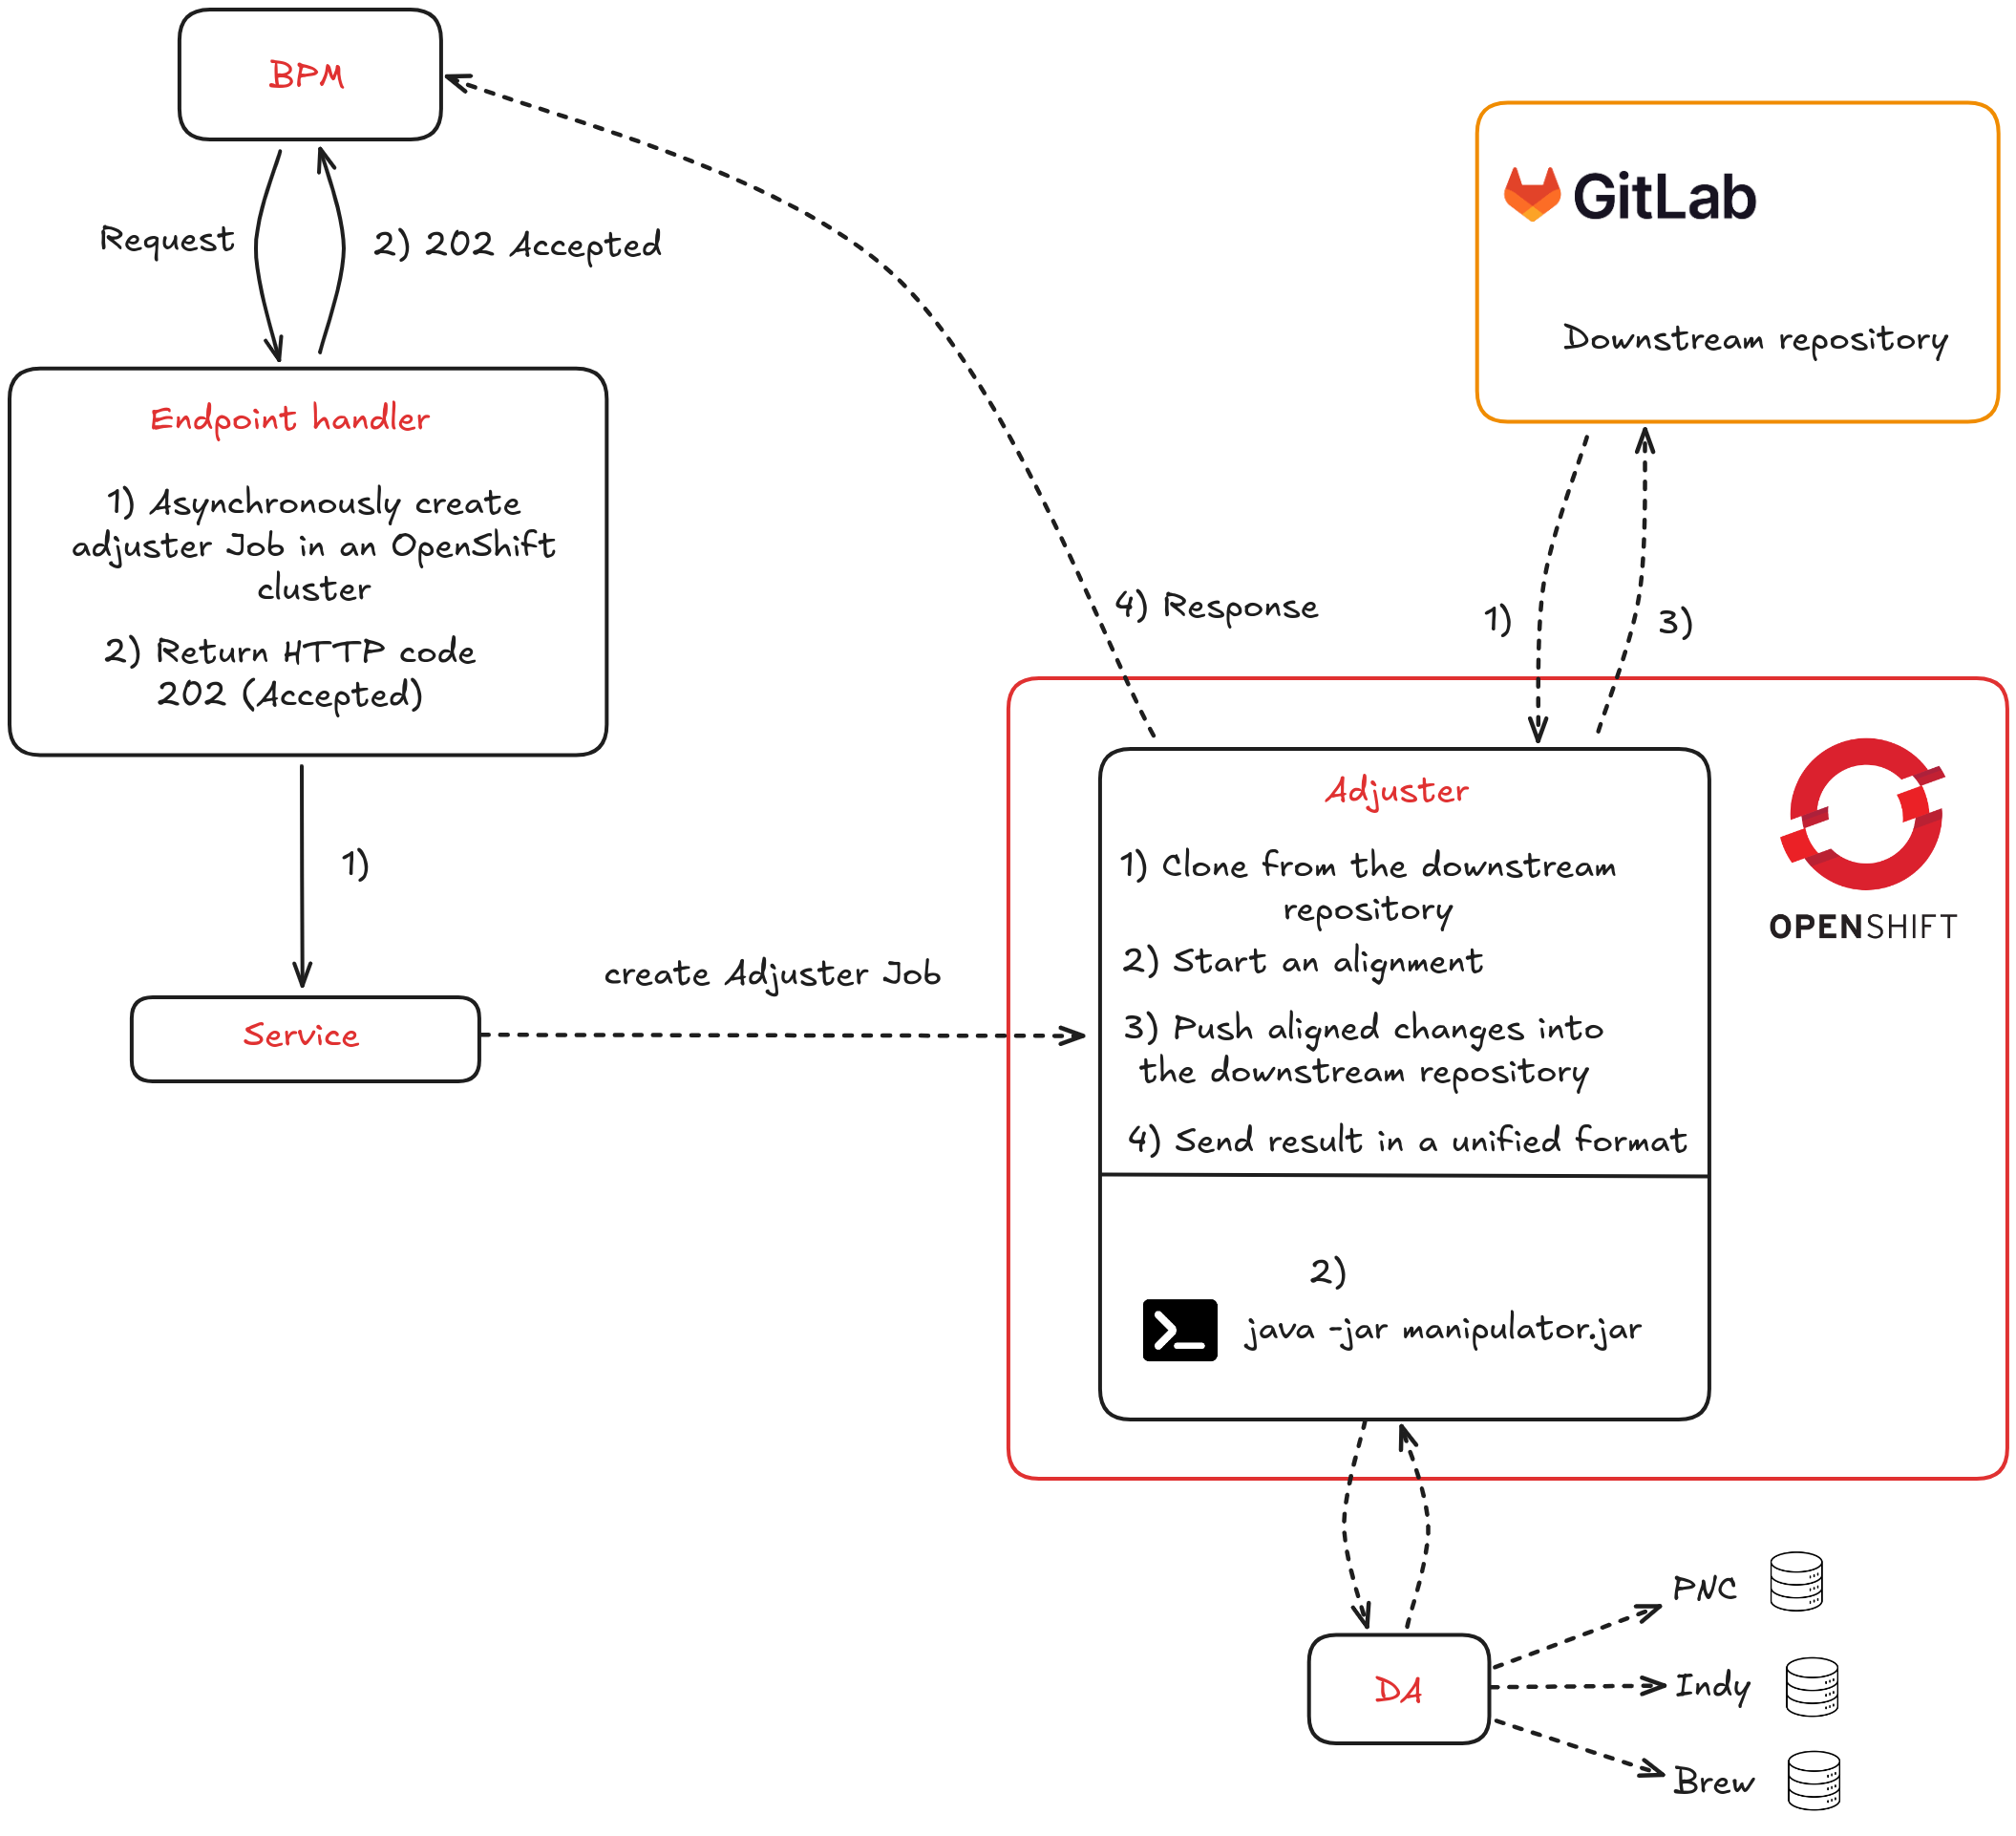
\includegraphics[width=\textwidth]{images/alignment-design.png}
  \end{center}
  \caption{Design of the alignment operation}
  \label{fig:alignment-design}
\end{figure}

\end{document}
